% id: 0514
% book: RPM 중3-2 수학 · 04 원주각
% section: 중단원 마무리하기
% figure: crop:fig-0514.png
% answer: ③
% answer_source: 답지
% variant_level: 0 (원본 전사)
% 이 파일은 build.mjs 가 items.json 에서 만든다. 고칠 때는 items.json 을 고친다.
\noindent\begin{minipage}[t]{0.58\linewidth}\vspace{0pt}\raggedright 오른쪽 그림에서 두 원~$\pt{O}$, $\pt{O'}$은 두 점~$\pt{A}$, $\pt{B}$에서 만나고 직선~$\pt{TT'}$은 점~$\pt{P}$를 접점으로 하는 원~$\pt{O}$의 접선이다. $\angle\pt{ADC}=70^\circ$, $\angle\pt{BCD}=62^\circ$일 때, $\angle x$의 크기는?\end{minipage}\hfill\begin{minipage}[t]{0.4\linewidth}\vspace{0pt}\centering \setlength{\dmfigw}{96.1pt}\ifdim\dmfigw>\linewidth\setlength{\dmfigw}{\linewidth}\fi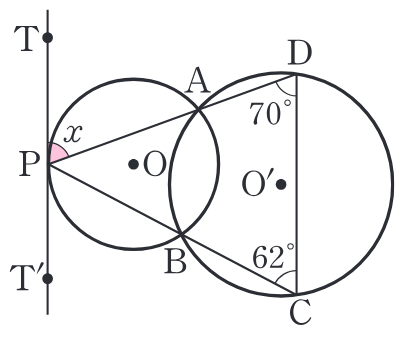
\includegraphics[width=\dmfigw]{figures/fig-0514.png}\end{minipage}\par
\dmchoicesauto{}{$68^\circ$}{$69^\circ$}{$70^\circ$}{$71^\circ$}{$72^\circ$}
